\documentclass{beamer}\usepackage[]{graphicx}\usepackage[]{color}
%% maxwidth is the original width if it is less than linewidth
%% otherwise use linewidth (to make sure the graphics do not exceed the margin)
\makeatletter
\def\maxwidth{ %
  \ifdim\Gin@nat@width>\linewidth
    \linewidth
  \else
    \Gin@nat@width
  \fi
}
\makeatother

\definecolor{fgcolor}{rgb}{0.345, 0.345, 0.345}
\newcommand{\hlnum}[1]{\textcolor[rgb]{0.686,0.059,0.569}{#1}}%
\newcommand{\hlstr}[1]{\textcolor[rgb]{0.192,0.494,0.8}{#1}}%
\newcommand{\hlcom}[1]{\textcolor[rgb]{0.678,0.584,0.686}{\textit{#1}}}%
\newcommand{\hlopt}[1]{\textcolor[rgb]{0,0,0}{#1}}%
\newcommand{\hlstd}[1]{\textcolor[rgb]{0.345,0.345,0.345}{#1}}%
\newcommand{\hlkwa}[1]{\textcolor[rgb]{0.161,0.373,0.58}{\textbf{#1}}}%
\newcommand{\hlkwb}[1]{\textcolor[rgb]{0.69,0.353,0.396}{#1}}%
\newcommand{\hlkwc}[1]{\textcolor[rgb]{0.333,0.667,0.333}{#1}}%
\newcommand{\hlkwd}[1]{\textcolor[rgb]{0.737,0.353,0.396}{\textbf{#1}}}%
\let\hlipl\hlkwb

\usepackage{framed}
\makeatletter
\newenvironment{kframe}{%
 \def\at@end@of@kframe{}%
 \ifinner\ifhmode%
  \def\at@end@of@kframe{\end{minipage}}%
  \begin{minipage}{\columnwidth}%
 \fi\fi%
 \def\FrameCommand##1{\hskip\@totalleftmargin \hskip-\fboxsep
 \colorbox{shadecolor}{##1}\hskip-\fboxsep
     % There is no \\@totalrightmargin, so:
     \hskip-\linewidth \hskip-\@totalleftmargin \hskip\columnwidth}%
 \MakeFramed {\advance\hsize-\width
   \@totalleftmargin\z@ \linewidth\hsize
   \@setminipage}}%
 {\par\unskip\endMakeFramed%
 \at@end@of@kframe}
\makeatother

\definecolor{shadecolor}{rgb}{.97, .97, .97}
\definecolor{messagecolor}{rgb}{0, 0, 0}
\definecolor{warningcolor}{rgb}{1, 0, 1}
\definecolor{errorcolor}{rgb}{1, 0, 0}
\newenvironment{knitrout}{}{} % an empty environment to be redefined in TeX

\usepackage{alltt}
\usepackage{amsfonts} % Worcester's
\usepackage{amssymb, amsfonts, latexsym, amsmath}
\usepackage{multirow,array,graphicx,rotating,epsfig}
\usepackage{verbatim}
\usepackage{enumerate}
\usepackage{color}
\usepackage{multicol}
\usepackage{subfig}
\usepackage{float}

%\usepackage{hyperref}

\hypersetup{
colorlinks=true,
urlcolor=cyan,
linkcolor=blue  
}

\newcommand{\ba}{{\bf a}}
\newcommand{\bA}{{\bf A}}
\newcommand{\mcA}{{\mathcal A}}
\newcommand{\bB}{{\bf B}}
\newcommand{\bb}{{\bf b}}
\newcommand{\mfB}{{\mathfrak B}}
\newcommand{\mcB}{{\mathcal B}}
\newcommand{\bc}{{\bf c}}
\newcommand{\bC}{{\bf C}}
\newcommand{\mcC}{{\mathcal C}}
\newcommand{\mbC}{{\mathbb C}}
\newcommand{\mcD}{{\mathcal D}}
\newcommand{\be}{{\bf e}}
\newcommand{\bE}{{\bf E}}
\newcommand{\mcF}{{\mathcal F}}
\newcommand{\mcG}{{\mathcal G}}
\newcommand{\bh}{{\bf h}}
\newcommand{\bH}{{\bf H}}
\newcommand{\mcH}{{\mathcal H}}
\newcommand{\mbH}{{\mathbb H}}
\newcommand{\mcI}{{\mathcal I}}
\newcommand{\bK}{{\bf K}}
\newcommand{\mcL}{{\mathcal L}}
\newcommand{\mcN}{{\mathcal N}}
\newcommand{\mcP}{{\mathcal P}}
\newcommand{\bq}{{\bf q}}
\newcommand{\bQ}{{\bf Q}}
\newcommand{\mbR}{{\mathbb R}}
\newcommand{\bR}{{\bf R}}
\newcommand{\mcS}{{\mathcal S}}
\newcommand{\mfS}{{\mathfrak S}}
\newcommand{\bs}{{\bf s}}
\newcommand{\mcT}{{\mathcal T}}
\newcommand{\bv}{{\bf v}}
\newcommand{\bV}{{\bf V}}
\newcommand{\mcV}{{\mathcal V}}
\newcommand{\bW}{{\bf W}}
\newcommand{\bw}{{\bf w}}
\newcommand{\bX}{{\bf X}}
\newcommand{\bx}{{\bf x}}
\newcommand{\bY}{{\bf Y}}
\newcommand{\bZ}{{\bf Z}}

\newcommand{\bzero}{{\bf 0}}
\newcommand{\bone}{{\bf 1}}

\newcommand{\bbeta}{{\boldsymbol{\beta}}}
\newcommand{\bep}{{\boldsymbol{\vep}}}
\newcommand{\bmu}{{\boldsymbol{\mu}}}
\newcommand{\vep}{\varepsilon}
\newcommand{\bvep}{{\boldsymbol{\vep}}}
%\newcommand{\bVep}{{\boldsymbol{\Varepsilon}}}
\newcommand{\bLambda}{{\boldsymbol{\Lambda}}}
\newcommand{\bPhi}{{\boldsymbol{\varPhi}}}
\newcommand{\bSigma}{{\boldsymbol{\Sigma}}}
\newcommand{\bxi}{{\boldsymbol{\xi}}}
\newcommand{\bXi}{{\boldsymbol{\Xi}}}

\DeclareMathOperator\E{E}
\DeclareMathOperator\Cov{Cov}
\DeclareMathOperator\Corr{Corr}
\DeclareMathOperator\diag{diag}
\DeclareMathOperator\logit{logit}
\DeclareMathOperator\sign{sign}
\DeclareMathOperator\Span{span}
\DeclareMathOperator\vc{vec}
\DeclareMathOperator\Var{Var}
\DeclareMathOperator\trace{trace}

\DeclareMathOperator\convD{\overset{\mcD}{\to}}
\DeclareMathOperator\convP{\overset{\mcP}{\to}}
\DeclareMathOperator\convas{\overset{as}{\to}}



%%%%%% Beamer Options
%\useoutertheme{infolines}
\definecolor{PSUblue}{RGB}{0,48,135}
\beamertemplatenavigationsymbolsempty
\setbeamerfont{page number in head/foot}{size=\small}
\setbeamertemplate{footline}[frame number]
%\addtobeamertemplate{headline}{}{\rule{\paperwidth}{3pt}}
\makeatletter
\def\th@mystyle{%
    \normalfont % body font
    \setbeamercolor{block title example}{bg=PSUblue,fg=white}
    \setbeamercolor{block body example}{bg=PSUblue!20,fg=black}
    \def\inserttheoremblockenv{exampleblock}
}
\makeatother
\theoremstyle{mystyle}
\newtheorem{mytheorem}{Theorem}


%%%%%% Knitr Options
\usepackage{etoolbox} 
\makeatletter 
\preto{\@verbatim}{\topsep=0pt \partopsep=0pt } 
\makeatother



%%
\IfFileExists{upquote.sty}{\usepackage{upquote}}{}
\begin{document}
%% \SweaveOpts{concordance=TRUE}
%% <<echo=FALSE,results='hide',message=FALSE>>=
%% opts_knit$set(width=20,out.width=20)
%% options(width=50)
%% library(fda)
%% library(refund)
%% set.seed(2016)
%% @

\title{
STAT 380: Week 1
}
\author{Instructor: Murali Haran Professor of Statistics\\ TA: Alex Zhao, PhD Student
}
\date{}

\begin{frame}
\titlepage
\end{frame}


\begin{frame}{Outline}
\begin{itemize}
\item Use the computer expressively to prepare, explore, and analyze data
\item Work closely with original raw data 
\item Use existing software rather than build routines from the ground up.
\item Focus on aspects of computing to conduct statistical analysis, NOT the computational aspects of statistical methods (For that: STAT 440, Computational Statistics)
\item Book: 
  \begin{itemize}
  \item Data Technologies and Computational Reasoning by D. Nolan and D. Temple Lang (pdf files will be posted weekly).
  \item Supplement: {\it Data Science in R: A Case Studies Approach to Computational Reasoning} by Nolan and Temple Lang.
  \end{itemize}
\end{itemize}
(With thanks to Professor Nolan for lecture notes)
\end{frame}

\begin{frame}{What are data?}
\begin{itemize}
\item Data are recorded/measured observations together with context. 

\item By context we mean the details of who, what, where, when, and/or how the observations were obtained, aka "metadata".
\end{itemize}

\end{frame}

\begin{frame}%{Tables of numbers}

\begin{center}
    {{\resizebox*{1.1\textwidth}{1.1\textheight}
        {\rotatebox{0}{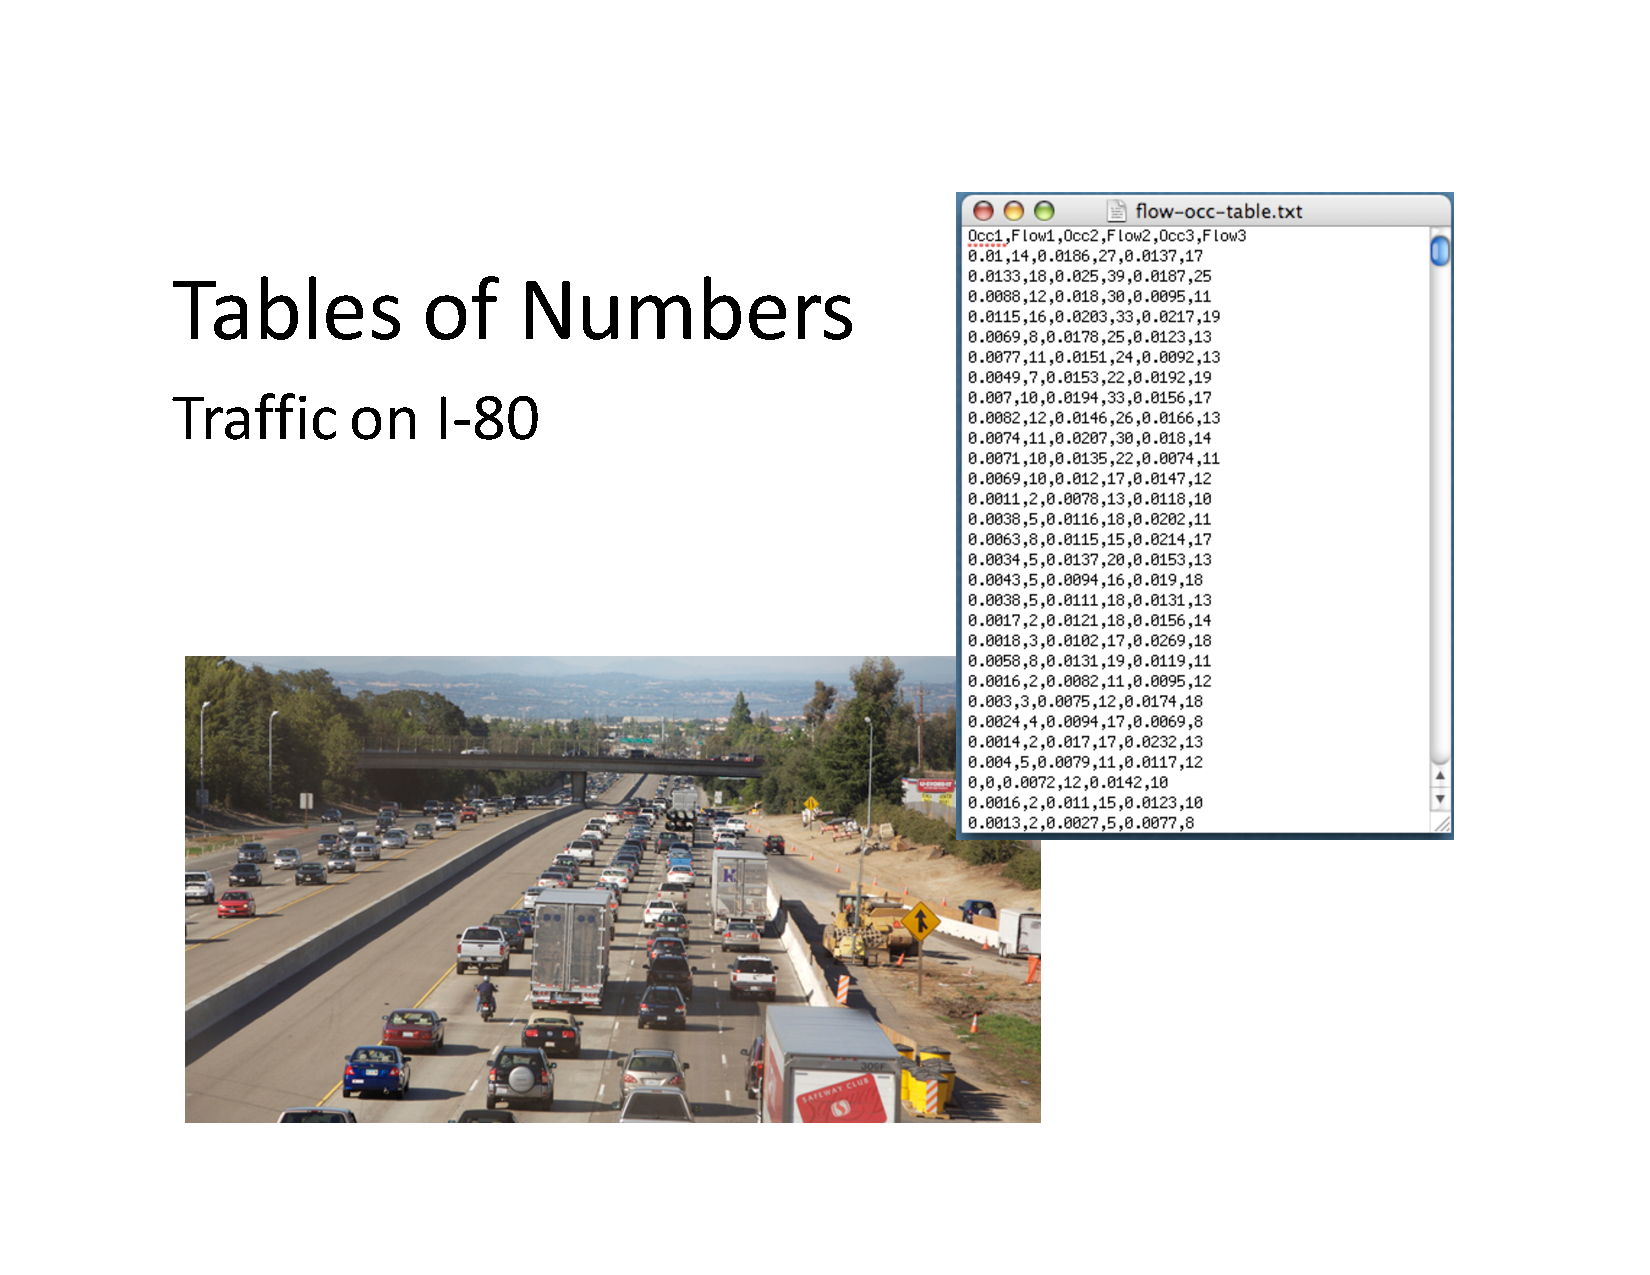
\includegraphics{trafficI80.pdf}}}} \par}
  \end{center}
\end{frame}

\begin{frame}%{GeographicInfo}

\begin{center}
    {{\resizebox*{1.1\textwidth}{1.1\textheight}
        {\rotatebox{0}{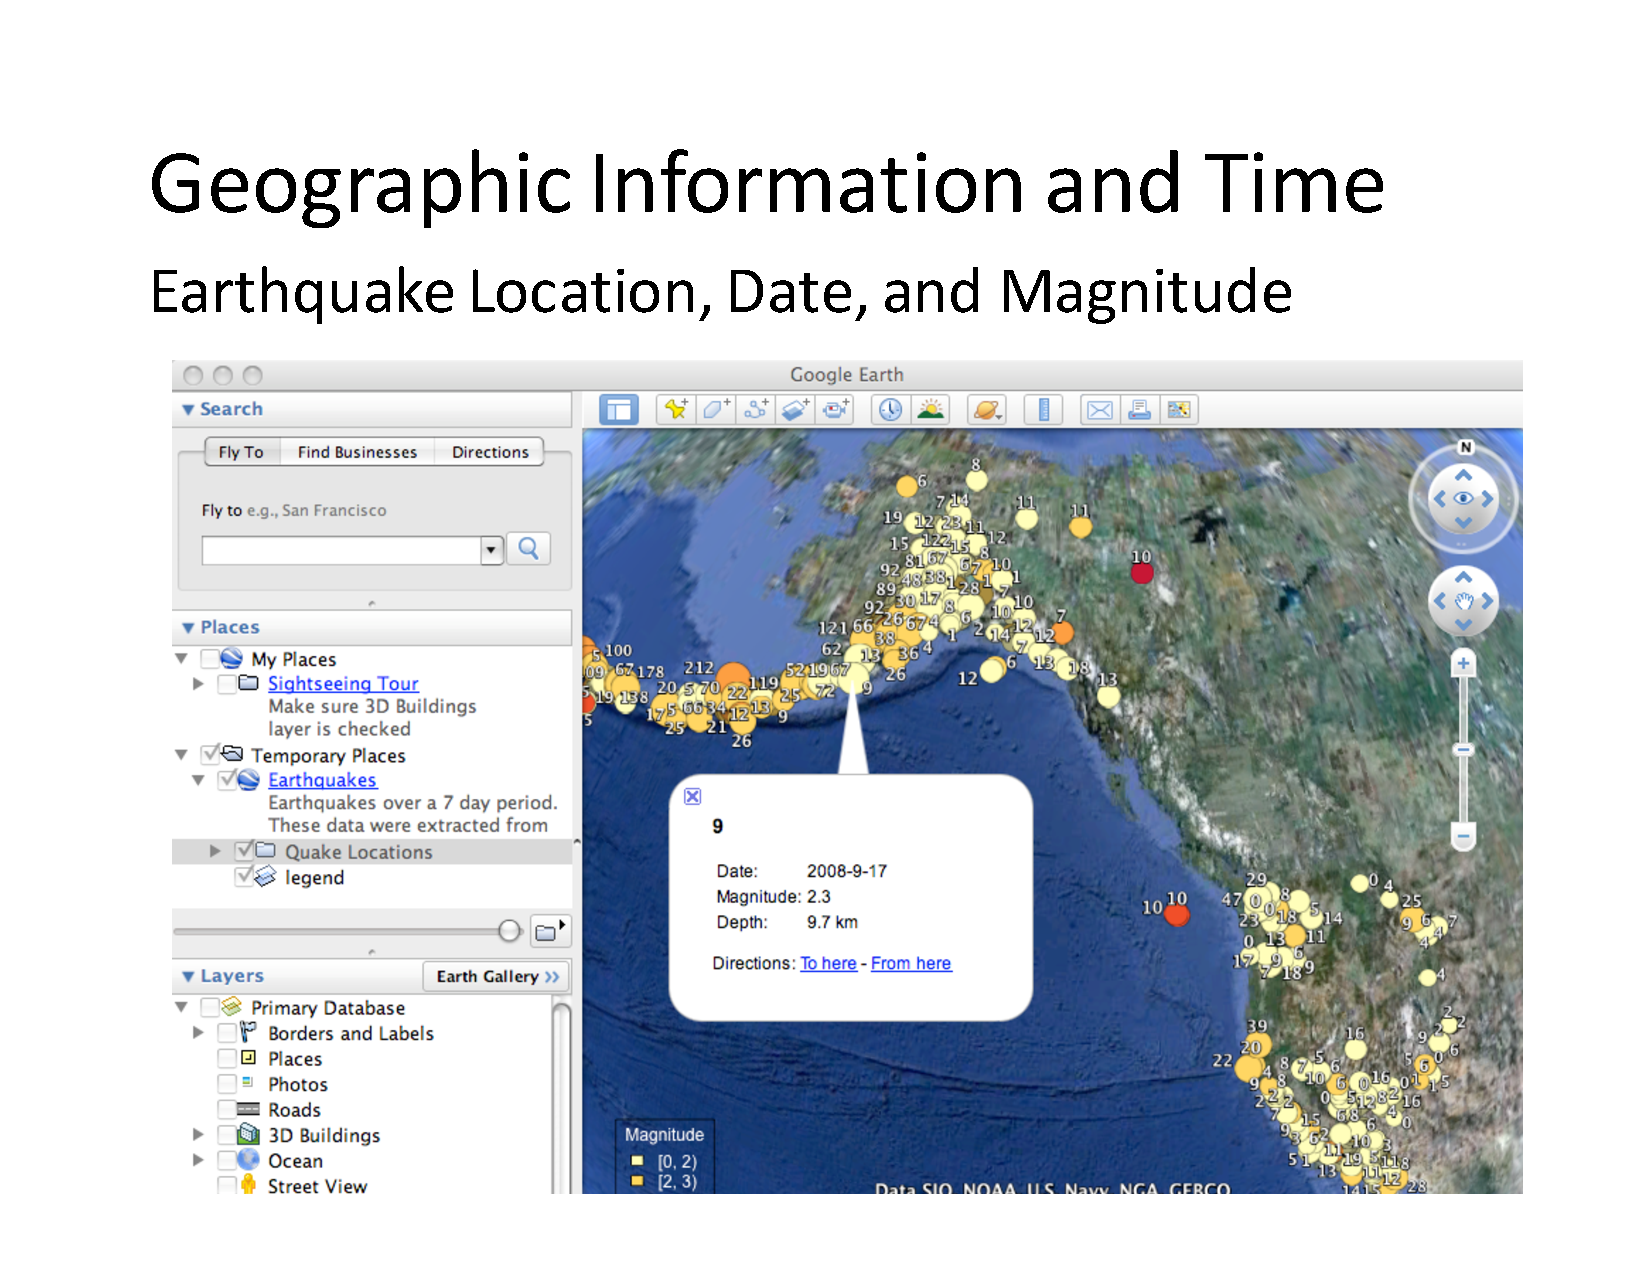
\includegraphics{Earthquake.pdf}}}} \par}
  \end{center}
\end{frame}
\begin{frame}%{Text}

\begin{center}
    {{\resizebox*{1.1\textwidth}{1.1\textheight}
        {\rotatebox{0}{
\includegraphics{Text.pdf}}}} \par}
  \end{center}
\end{frame}
\begin{frame}%{Graph}

\begin{center}
    {{\resizebox*{1.1\textwidth}{1.1\textheight}
        {\rotatebox{0}{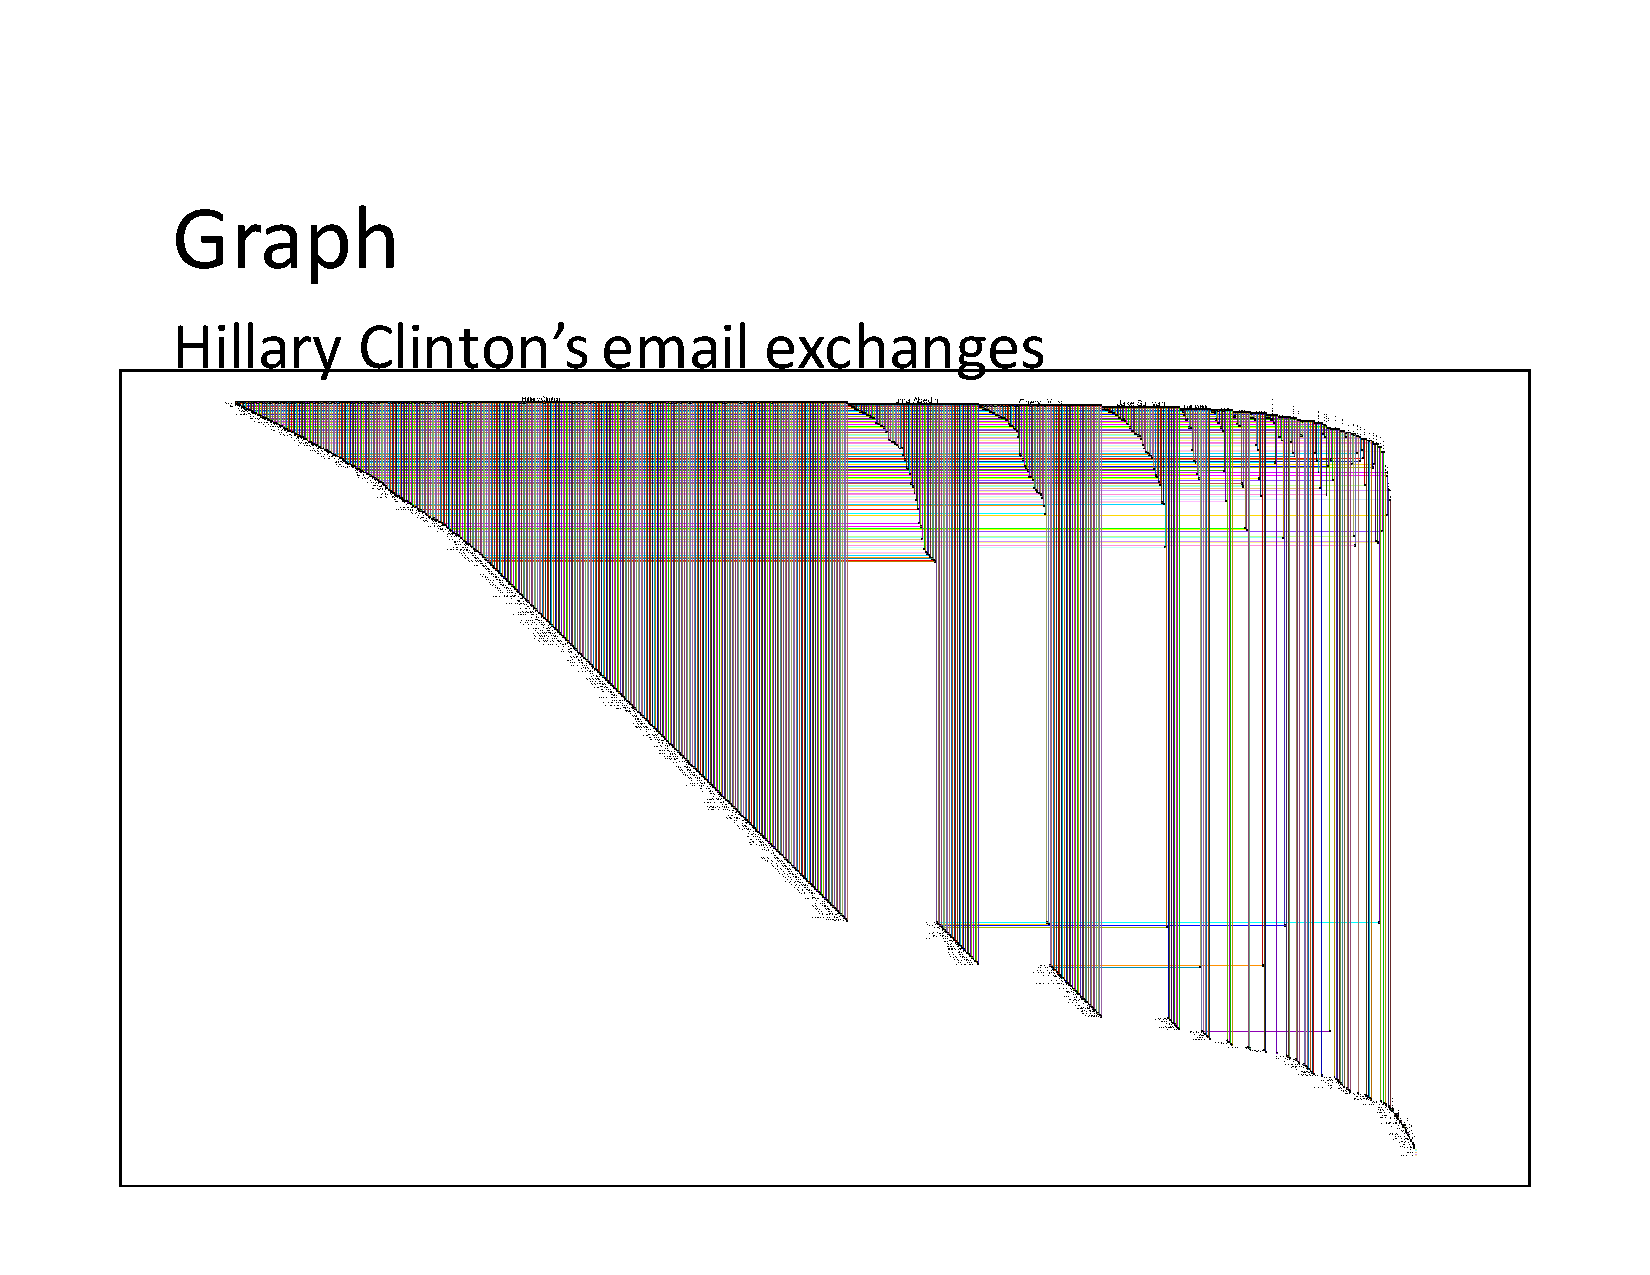
\includegraphics{Graph.pdf}}}} \par}
  \end{center}
\end{frame}
\begin{frame}%{Metadata}

\begin{center}
    {{\resizebox*{1.1\textwidth}{1.1\textheight}
        {\rotatebox{0}{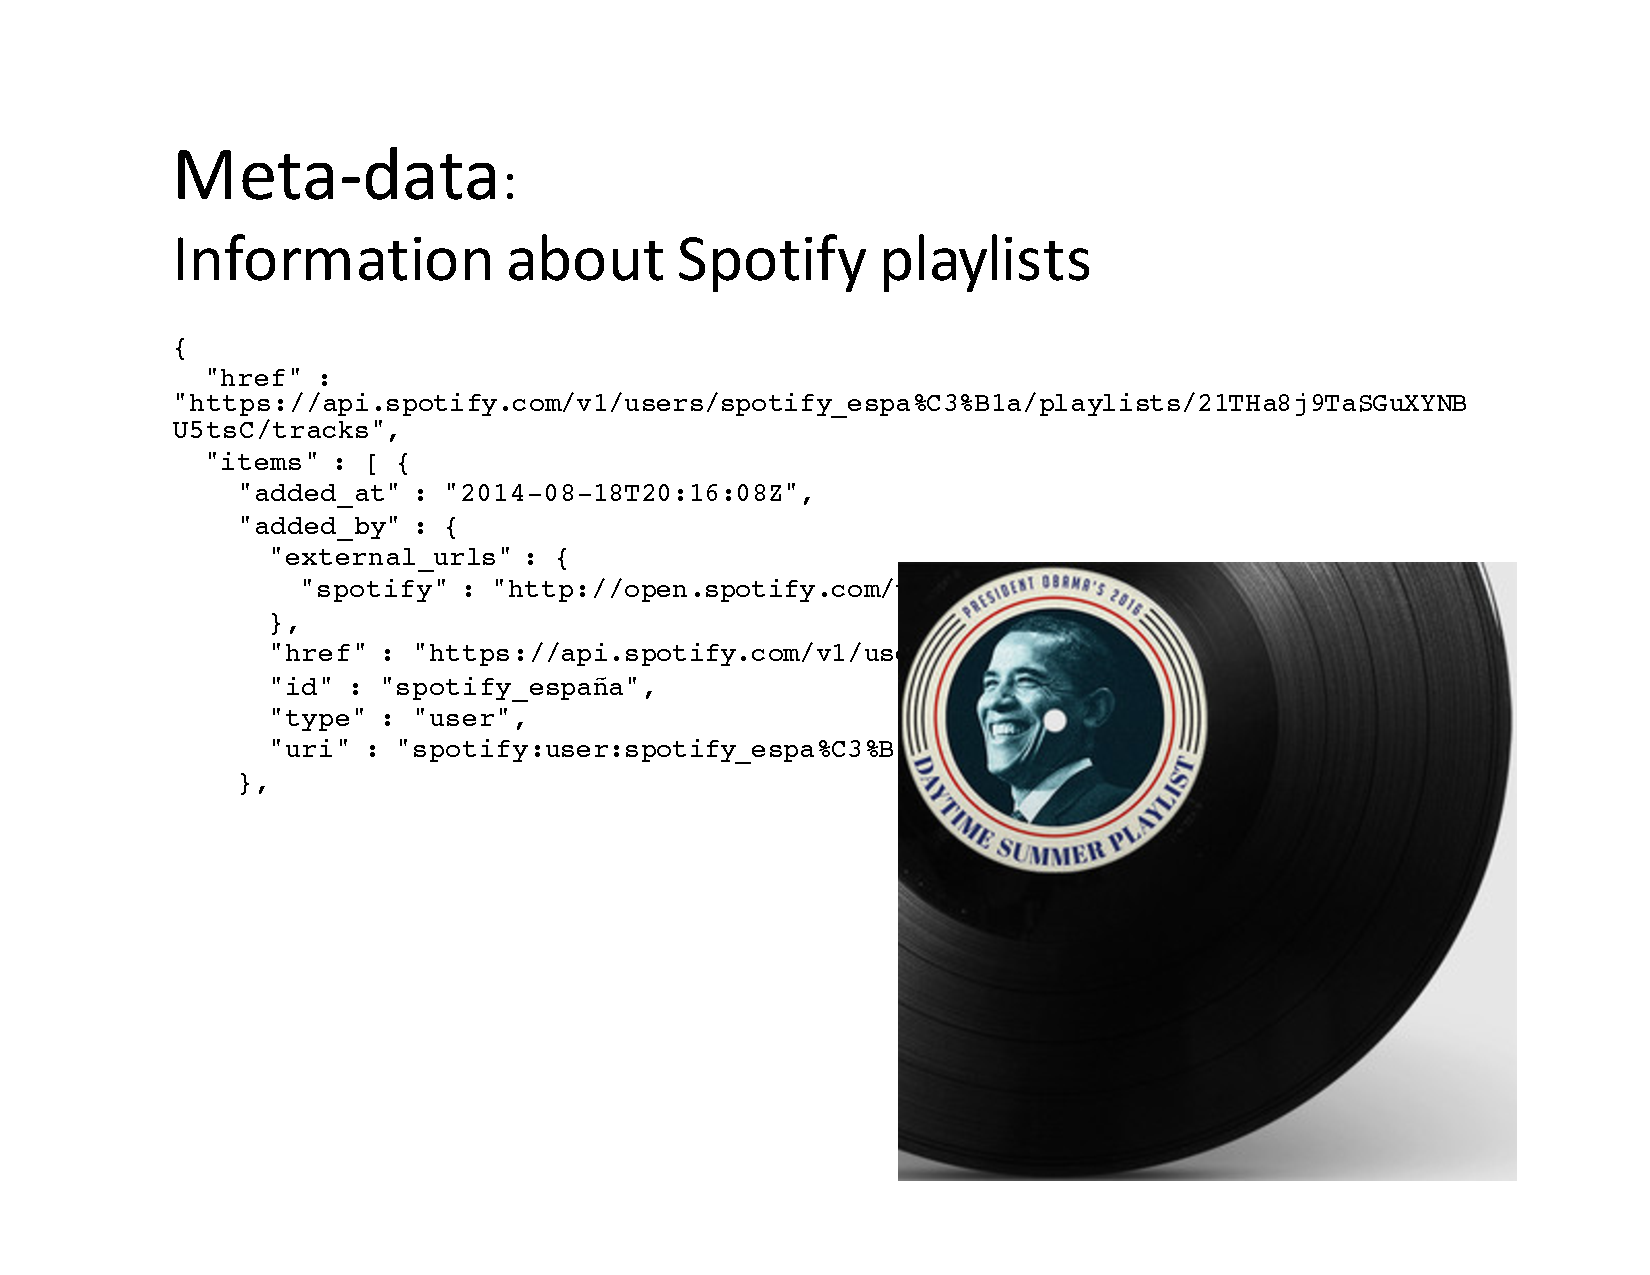
\includegraphics{Metadata.pdf}}}} \par}
  \end{center}
\end{frame}
\begin{frame}%{Image}

\begin{center}
    {{\resizebox*{1.1\textwidth}{1.1\textheight}
        {\rotatebox{0}{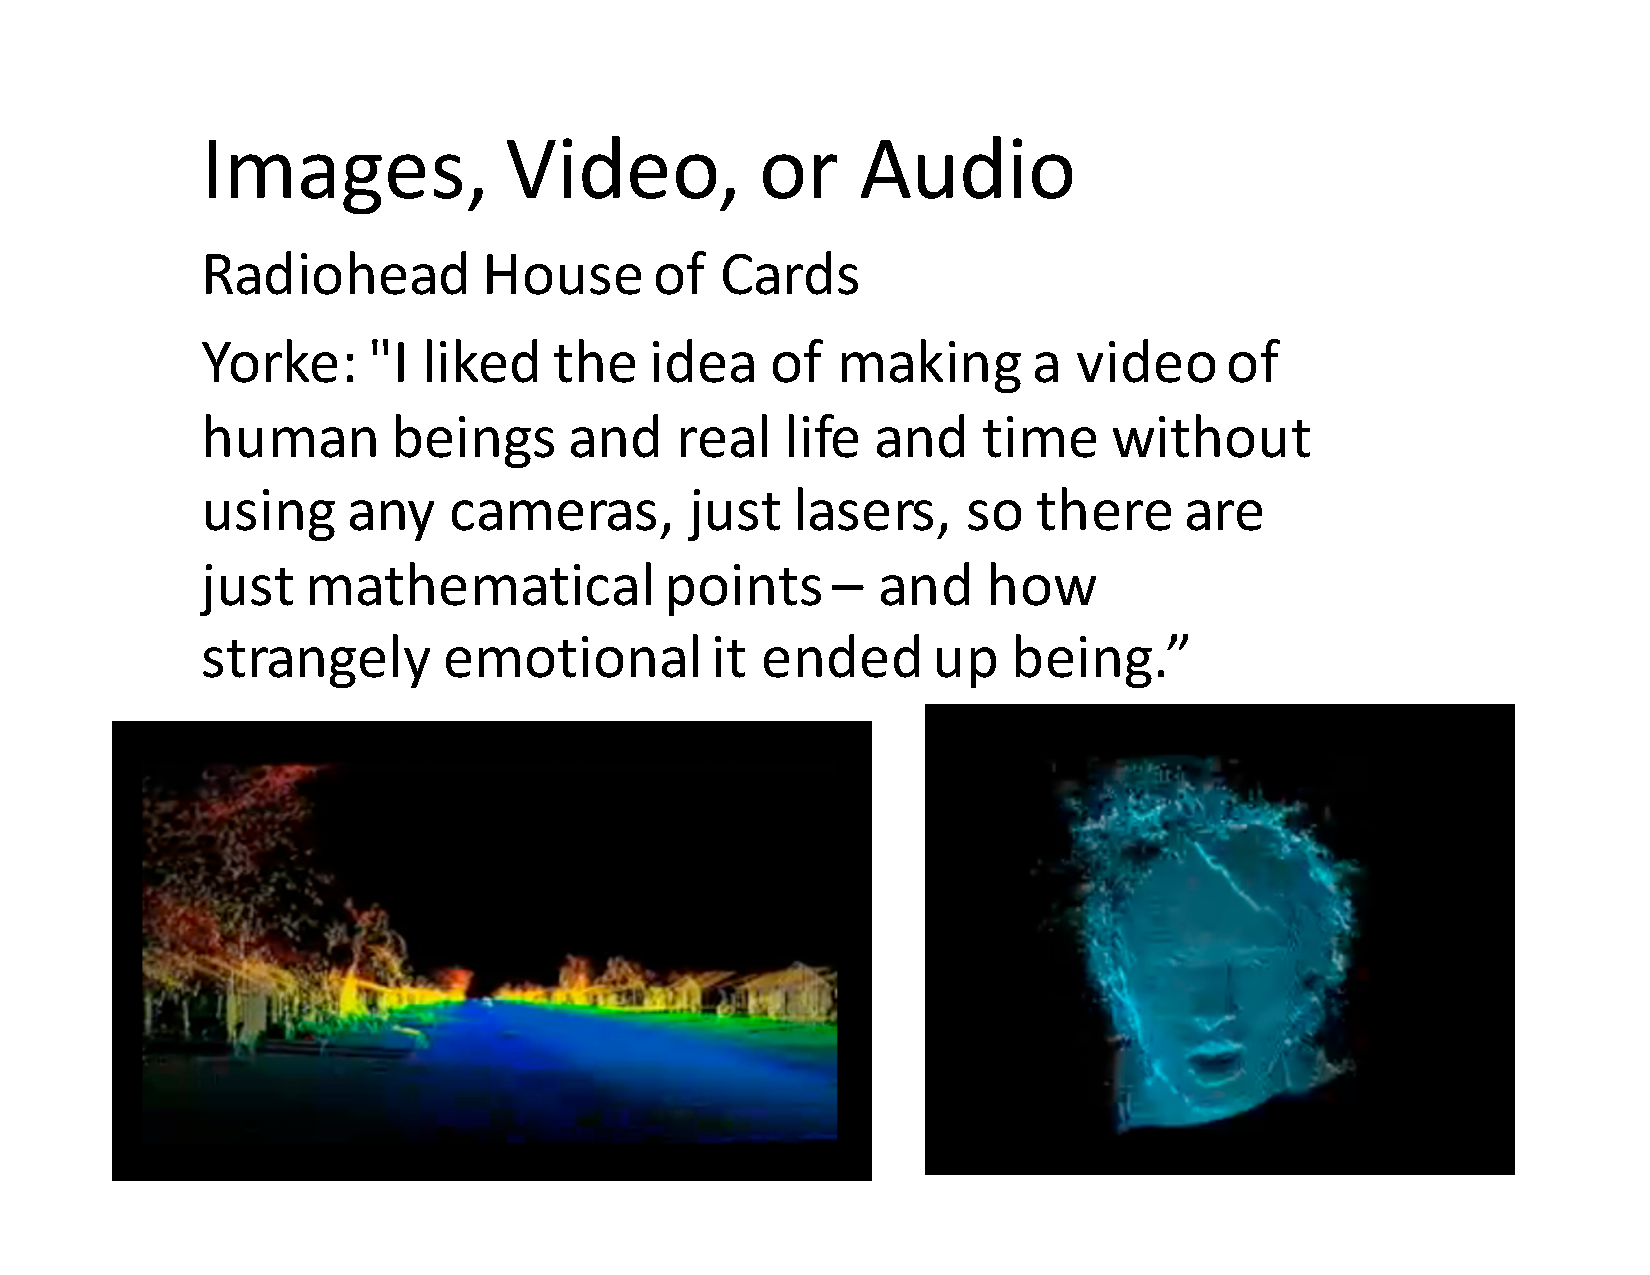
\includegraphics{Image.pdf}}}} \par}
  \end{center}
\end{frame}

\begin{frame}{What does a data scientist do?}
AIG job posting on Kaggle for senior data scientist:
\begin{itemize}
\item Build predictive models utilizing both traditional statistical methods and modern machine learning techniques 
\item Extract, clean, and manipulate large datasets (structured and unstructured) for model building.
\item Communicate (written and verbal) insights from quantitative analyses to technical and non-technical audiences. 
\item Stay current on the latest machine learning and big data trends.
\item Work with business sponsors and IT teams to implement analytic solutions.
\item Serve as a technical expert on one or more domains (e.g. Time Series Analysis, Text Mining, etc.) 
\end{itemize}
\end{frame}

\begin{frame}{What Skills does a Data Scientist need?}
AIG job postings on Kaggle
\begin{itemize}
\item Expertise in at least one modeling/machine learning platform such as R, Python, or SAS. 
\item Knowledge of an additional general purpose programming language such as C++ or Java. 
\item Advanced SQL skills and experience with No SQL technologies.
\item Built several predictive models that have been put into live production. 
\item Obsess over sample bias, over-fitting, variable selection, missing values, etc.
\item Understand the need to balance predictive power, interpretability, and ease of implementation
\end{itemize}
\end{frame}

\begin{frame}{Data analysis cycle}
\begin{itemize}
\item Data ACQUISITION – Input/output, regular expressions 
\item Data CLEANING – verification, manipulation
\item Data ORGANIZATION – data frames, data bases, XML
\item Data EXPLORATION – search for interesting patterns
\item Data VISUALIZATION – create statistical graphs
\item Data ANALYSIS – fit and assess statistical models 
\item Data SIMULATION – studies of random behavior
\item Data REPORTING – report findings from analysis
\end{itemize}
\end{frame}

\begin{frame}{Statistical concepts}
\begin{itemize}
\item Basic numeracy: Variability, Patterns, comparisons
\item Exploratory Data Analysis
\item Graphics: Elements and principles of graphing 
\item Computationally intensive methods, e.g.,
Classification and Regression trees, multi-dimensional scaling, nearest neighbor method
\item Simulation tools: Monte Carlo, bootstrap, cross-validation
\end{itemize}
\end{frame}

\begin{frame}{Computing concepts}
\begin{itemize}
\item Programming concepts
Control flow
trees
functions
\item Regular expressions and text manipulation 
\item Relational databases
\item Random number generation
\item Representation of information in the computer 
\end{itemize}
\end{frame}

\begin{frame}{Software}
\begin{itemize}
\item R – statistical software
\item SQL – structured query language for relational databases
\item XML – Extensible Markup Language (and HTML) and XPath
\item Unix – shell commands
\end{itemize}
\end{frame}

\begin{frame}{Grading}
\begin{itemize}
  \item Homework + projects: add up to 50\%. Exact proportion may
    change. {\it Tentatively}:
    \begin{itemize}
    \item Homework = 35\% %30\% + Projects = 20\%
    \end{itemize}
    \item Homework due in class. After class, before 3:30pm (in my mailbox in Thomas 326): 20\% off. After that, 0 credit no matter what.
  \item Drop two lowest homework scores. 
  \item Midterm: 25\%
  \item Final: 40\%
\end{itemize}
\end{frame}

\begin{frame}{Academic integrity}
\begin{itemize}
\item Free to discuss course matters with instructor, TA, and fellow students
\item DO NOT SHARE CODE 
\item Make significant contribution to your group’s work
\item If you are uncertain as to whether something may be a violation of the code, ask the instructor 
\item Writing a program is like writing a paper – your code should be your original work.  
\item A violation will result in at least one of the following:
0 on the assignment, 
F for the course grade, 
Report to the Office of Student Conduct
\end{itemize}
\end{frame}

%% \begin{frame}{Example - Canadian Weather}
%% One of the most often used data sets in FDA is actually spatial.
%% <<echo=FALSE,fig.height=5>>=
%% par(mar=c(4,4,1,1))
%% Y = CanadianWeather$dailyAv[,,1]
%% times = seq(0,1,length=365)
%% matplot(times,Y,type="l",ylab="Temp C",xlab="Day of Year",xlim=c(0,1),ylim=c(-40,25))
%% vl = cumsum(c(0,31,28,31,30,31,30,31,31,30,31,30,31))/365
%% m_pts = (vl[-1] + vl[-13])/2
%% mts<-c("J","F","M","A","M","J","J","A","S","O","N","D")
%% abline(v=vl,lty=2,col="grey")
%% text(x=m_pts,y=-39,labels=mts,cex=1.5)
%% @
%% \end{frame}


\end{document}



